\documentclass[12pt]{article}
\usepackage[margin=1in]{geometry}
\usepackage[colorlinks=true]{hyperref}
\usepackage{parskip}

\usepackage{tikz}
\usetikzlibrary{calc}
\usetikzlibrary{decorations.markings}
\usetikzlibrary{positioning}

\begin{document}

We sketch a variety of methods for drawing string diagrams (aka wiring
diagrams) in TikZ. An important requirement is that the method be
\emph{automatable}: we should be able to generate the TikZ code mechanically,
without human tweaking.

\section*{Automatic layout: graph drawing}

\usetikzlibrary{graphdrawing}
\usetikzlibrary{graphs}
\usegdlibrary{layered}

A first approach is to use the TikZ graph drawing library
(\texttt{graphdrawing}). The ``layered layout'' uses the \emph{Sugiyama
  method}, the same algorithm used by Graphviz's \texttt{dot} program.

\paragraph{Graph edges}

The anchors in \texttt{graphdrawing} are not normal anchors. They are either
strings (``center'' or a compass direction like ``north east'') or numbers
(angles in  degrees from positive x-axis). In particular, it is not possible to
refer by name to arbitrary anchors of custom shapes.

See (TikZ Manual, \S 27.8, ``Anchoring Edges'') and also the call to Lua
function \texttt{createVertex} in the TikZ
\href{http://pgf.cvs.sourceforge.net/viewvc/pgf/pgf/generic/pgf/graphdrawing/tex/pgflibrarygraphdrawing.code.tex?view=markup}{source code}.

\begin{center}
\begin{tikzpicture}[decoration={
    markings,
    mark=at position 0.5 with {\arrow{>}}}
    ] 
  \graph[layered layout,edges={postaction={decorate}},
         nodes={rectangle,draw},math nodes,
         grow'=right,layer distance=4em,sibling sep=2em]{
    f0/"" [draw=none];
    g0/"" [draw=none];
    f [minimum height=2em];
    g [minimum height=2em];
    h [minimum height=4em];
  
    f0 --[edge label=$A$] f;
    g0 --[edge label=$B$] g;
    f --[edge node={node [above,midway] {$A$}}, tail anchor=0, head anchor=135] h;
    g --[edge node={node [above,midway] {$B$}}, tail anchor=0, head anchor=225] h;
  };
\end{tikzpicture}
\end{center}

\paragraph{Standard edges}

Inspired by \href{http://tex.stackexchange.com/a/247825}{TeX.SE}, I think it's
better to use invisible edges in \texttt{graphdrawing} and then draw the edges
manually using the standard \texttt{\textbackslash draw} macro in TikZ.

\begin{center}
\begin{tikzpicture}[decoration={
    markings,
    mark=at position 0.5 with {\arrow{>}}}
    ] 
  \graph[layered layout,edges={draw=none},nodes={rectangle,draw},math nodes,
         grow'=right,layer distance=4em,sibling sep=1em]{
    f [minimum height=2em];
    g [minimum height=2em];
    h [minimum height=5em];
    
    f -> h;
    g -> h;
  };
  
  \coordinate (h_in1) at ($(h.north west)!0.33!(h.south west)$);
  \coordinate (h_in2) at ($(h.north west)!0.66!(h.south west)$);
  \coordinate (h_out1) at ($(h.north east)!0.33!(h.south east)$);
  \coordinate (h_out2) at ($(h.north east)!0.66!(h.south east)$);
  
  \draw[postaction={decorate}] (f) -> (h_in1) node [above,midway] {$A$};
  \draw[postaction={decorate}] (g) -> (h_in2) node [above,midway] {$B$};

  \draw[postaction={decorate}] ($(f)-(4em,0)$) -> (f) node [above,midway] {$A$};
  \draw[postaction={decorate}] ($(g)-(4em,0)$) -> (g) node [above,midway] {$B$};
  \draw[postaction={decorate}] (h_out1) -> ($(h_out1)+(4em,0)$) node [above,midway] {$X$};
  \draw[postaction={decorate}] (h_out2) -> ($(h_out2)+(4em,0)$) node [above,midway] {$X$};
\end{tikzpicture}
\end{center}

Alternatively, with curved edges:

\begin{center}
\begin{tikzpicture}[decoration={
    markings,
    mark=at position 0.5 with {\arrow{>}}},
    % http://tex.stackexchange.com/a/5496/124082
    execute at begin node=$, execute at end node=$
    ] 
  \graph[layered layout,edges={draw=none},nodes={rectangle,draw},
         grow'=right,layer distance=4em,sibling sep=1em]{
    in1/"" [draw=none];
    in2/"" [draw=none];
    out1/"" [draw=none];
    out2/"" [draw=none];
    f [minimum height=2em];
    g [minimum height=2em];
    h [minimum height=4em];

    in1 -> f;
    in2 -> g;
    f -> h;
    g -> h;
    h -> out1;
    h -> out2;
  };
  
  \coordinate (h_in1) at ($(h.north west)!0.33!(h.south west)$);
  \coordinate (h_in2) at ($(h.north west)!0.66!(h.south west)$);
  \coordinate (h_out1) at ($(h.north east)!0.33!(h.south east)$);
  \coordinate (h_out2) at ($(h.north east)!0.66!(h.south east)$);
    
  \draw[postaction={decorate}] (f) to[out=0,in=180] node[above] {A} (h_in1);
  \draw[postaction={decorate}] (g) to[out=0,in=180] node[above] {B} (h_in2);

  \draw[postaction={decorate}] (in1) to node[above] {A} (f);
  \draw[postaction={decorate}] (in2) to node[above] {B} (g);
  \draw[postaction={decorate}] (h_out1) to[out=0,in=180] node[above] {X} (out1);
  \draw[postaction={decorate}] (h_out2) to[out=0,in=180] node[above] {X} (out2);
\end{tikzpicture}
\end{center}

While the graph layout is fine in this simple case, it fails on more
complicated examples. One reason is that the layout algorithm, particularly the
edge crossing heuristics, cannot account for the ``ports'' that we wish to
assign to nodes like $h$. (In contrast, Graphviz \emph{does} support ports
through its record and HTML labels.)

\section*{Semi-automatic layout: matrices}

We give up on automatic layout and try using the \texttt{matrix} library to
help with node alignment.

\usetikzlibrary{matrix}

\paragraph{One matrix} In this approach, we use a single matrix with one row
and a column for every composition. Inside each column, the nodes of the tensor
product are positioned essentially manually (using \texttt{below of}
directives).

\begin{center}
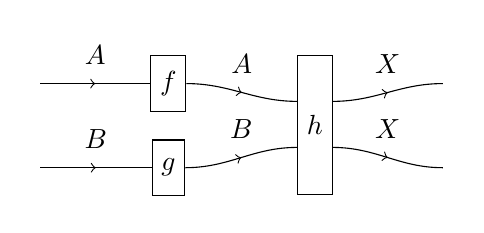
\begin{tikzpicture}[decoration={
    markings,
    mark=at position 0.5 with {\arrow{>}}},
    execute at begin node=$, execute at end node=$,
    every node/.style={minimum height=2em}
  ]
  \node[matrix,column sep=4em,anchor=north] (mat) {
    \node[inner sep=0] (in1) {};
    \node[inner sep=0, below=1em of in1] (in2) {};
    &
    \node[draw] (f) {f};
    \node[draw, below=1em of f] (g) {g};
    &
    \node[draw, minimum height=5em] (h) {h};
    &
    \node[inner sep=0] (out1) {};
    \node[inner sep=0, below=1em of out1] (out2) {};
    \\
  };

  \coordinate (h_in1) at ($(h.north west)!0.33!(h.south west)$);
  \coordinate (h_in2) at ($(h.north west)!0.66!(h.south west)$);
  \coordinate (h_out1) at ($(h.north east)!0.33!(h.south east)$);
  \coordinate (h_out2) at ($(h.north east)!0.66!(h.south east)$);
  
  \draw[postaction={decorate}] (in1) to node[above] {A} (f);
  \draw[postaction={decorate}] (in2) to node[above] {B} (g);
  \draw[postaction={decorate}] (f) to[out=0,in=180] node[above] {A} (h_in1);
  \draw[postaction={decorate}] (g) to[out=0,in=180] node[above] {B} (h_in2);
  \draw[postaction={decorate}] (h_out1) to[out=0,in=180] node[above] {X} (out1);
  \draw[postaction={decorate}] (h_out2) to[out=0,in=180] node[above] {X} (out2);
\end{tikzpicture}
\end{center}

\paragraph{Matrix columns} Dually, for every tensor of size $n$, we can create
a matrix with $n$ rows and one column. The compositions are positioned manually
(using \texttt{right of} directives on the matrix nodes). Ideally we would
combine this approach with the previous one, but it's not possible to nest
matrices in TikZ 3.0.

\begin{center}
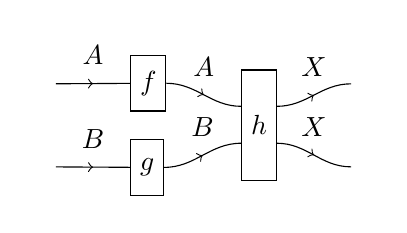
\begin{tikzpicture}[decoration={
    markings,
    mark=at position 0.5 with {\arrow{>}}},
    execute at begin node=$, execute at end node=$,
    every node/.style={minimum height=2em},
    every matrix/.style={row sep=1em}
  ]
  \node[matrix] (in) {
    \node (in1) {}; \\
    \node (in2) {}; \\
  };
  \node[matrix,right=2em of in] (m1) {
    \node[draw] (f) {f}; \\
    \node[draw] (g) {g}; \\
  };
  \node[matrix,right=2em of m1] (m2) {
    \node[draw, minimum height=4em] (h) {h}; \\
  };
  \node[matrix,right=2em of m2] (out) {
    \node (out1) {}; \\
    \node (out2) {}; \\
  };

  \coordinate (h_in1) at ($(h.north west)!0.33!(h.south west)$);
  \coordinate (h_in2) at ($(h.north west)!0.66!(h.south west)$);
  \coordinate (h_out1) at ($(h.north east)!0.33!(h.south east)$);
  \coordinate (h_out2) at ($(h.north east)!0.66!(h.south east)$);
  
  \draw[postaction={decorate}] (in1) to node[above] {A} (f);
  \draw[postaction={decorate}] (in2) to node[above] {B} (g);
  \draw[postaction={decorate}] (f) to[out=0,in=180] node[above] {A} (h_in1);
  \draw[postaction={decorate}] (g) to[out=0,in=180] node[above] {B} (h_in2);
  \draw[postaction={decorate}] (h_out1) to[out=0,in=180] node[above] {X} (out1);
  \draw[postaction={decorate}] (h_out2) to[out=0,in=180] node[above] {X} (out2);
\end{tikzpicture}
\end{center}

Here's another example:

\begin{center}
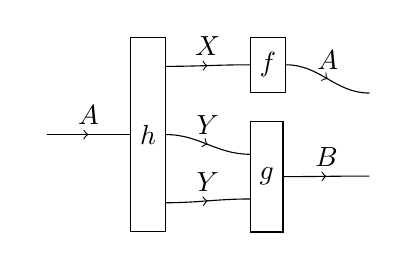
\begin{tikzpicture}[decoration={
    markings,
    mark=at position 0.5 with {\arrow{>}}},
    execute at begin node=$, execute at end node=$,
    every matrix/.style={
      inner sep=0, row sep=1em,
      nodes={inner sep=0.333em, minimum height=2em}
    }
  ]
  \node[matrix] (in) {
    \node (in1) {}; \\
  };
  \node[matrix, right=3em of in] (m1) {
    \node[draw, minimum height=7em] (h) {h}; \\
  };
  \node[matrix, right=3em of m1] (m2) {
    \node[draw] (f) {f}; \\
    \node[draw, minimum height=4em] (g) {g}; \\
  };
  \node[matrix, right=3em of m2] (out) {
    \node (out1) {}; \\
    \node (out2) {}; \\
  };

  \coordinate (h_out1) at ($(h.north east)!0.15!(h.south east)$);
  \coordinate (h_out2) at ($(h.north east)!0.50!(h.south east)$);
  \coordinate (h_out3) at ($(h.north east)!0.85!(h.south east)$);
  \coordinate (g_in1) at ($(g.north west)!0.30!(g.south west)$);
  \coordinate (g_in2) at ($(g.north west)!0.70!(g.south west)$);
  
  \draw[postaction={decorate}] (in1) to node[above] {A} (h);
  \draw[postaction={decorate}] (h_out1) to[out=0,in=180] node[above] {X} (f);
  \draw[postaction={decorate}] (h_out2) to[out=0,in=180] node[above] {Y} (g_in1);
  \draw[postaction={decorate}] (h_out3) to[out=0,in=180] node[above] {Y} (g_in2);
  \draw[postaction={decorate}] (f) to[out=0,in=180] node[above] {A} (out1);
  \draw[postaction={decorate}] (g) to[out=0,in=180] node[above] {B} (out2);
\end{tikzpicture}
\end{center}

\section*{Manual layout}

\usetikzlibrary{fit}

The potential of the matrix approach cannot be fully realized because TikZ does
not allow matrices to be nested. What we really want is \emph{compositional} or
\emph{functional} graphics, as in
\href{https://docs.racket-lang.org/pict/}{Pict} for Racket or
\href{https://github.com/GiovineItalia/Compose.jl}{Compose.jl} for Julia. TikZ
has a different programming model. We consider some ways to try to force the
compositional model onto TikZ.

\paragraph{Fit} The \texttt{fit} library creates nodes bounding arbitrary sets
of coordinates.

\begin{center}
\begin{tikzpicture}[decoration={
    markings,
    mark=at position 0.5 with {\arrow{>}}},
    execute at begin node=$, execute at end node=$,
    every node/.style={minimum height=2em}
  ]
  \node[draw] (f1) {f_1};
  \node[draw,right=2em of f1] (g1) {g_1};
  \draw[postaction={decorate}] (f1) to node[above] {X} (g1);
  \node[draw,dotted,fit=(f1) (g1)] (f1g1) {};

  \node[draw, below=1em of f1g1] (f2) {f_2};

  \node[fit=(f1g1) (f2)] (outer) {};
  \coordinate (outer_in1) at
    ($(outer.north west)!0.33!(outer.south west)-(2em,0)$);
  \coordinate (outer_in2) at
    ($(outer.north west)!0.66!(outer.south west)-(2em,0)$);
  \coordinate (outer_out1) at
    ($(outer.north east)!0.33!(outer.south east)+(2em,0)$);
  \coordinate (outer_out2) at
    ($(outer.north east)!0.66!(outer.south east)+(2em,0)$);
  
  \draw[postaction={decorate}] (outer_in1) to[out=0,in=180] node[above] {A} (f1);
  \draw[postaction={decorate}] (outer_in2) to[out=0,in=180] node[above] {A} (f2);
  \draw[postaction={decorate}] (g1) to[out=0,in=180] node[above] {B} (outer_out1);
  \draw[postaction={decorate}] (f2) to[out=0,in=180] node[above] {B} (outer_out2);
\end{tikzpicture}
\end{center}

The \texttt{fit} library is useful for drawing outer boxes, but it's utility
for layout is limited because you can only create a fitted box \emph{after} its
content has been placed on the canvas.

\paragraph{Pic} At first sight, the \texttt{pic} library looks like exactly
what the doctor ordered. It allows you to create ``small pictures'' that are
reusable and behave in many ways like nodes. However, a crucial difference is
that TikZ does not assign anchors to pics like it does to nodes. Consequently,
aligning pics is difficult:

\begin{center}
\begin{tikzpicture}[
    decoration={markings, mark=at position 0.5 with {\arrow{>}}},
    execute at begin node=$, execute at end node=$,
    every node/.style={minimum height=2em},
    f1g1/.pic={
      \node[draw] (f1) {f_1};
      \node[draw,right=2em of f1] (g1) {g_1};
      \draw[postaction={decorate}] (f1) to node[above,midway] {X} (g1);
    },
    f2g2/.pic={
      \node[draw] (f2) {\mathrm{foo}_2};
      \node[draw,right=2em of f2] (g2) {\mathrm{goo}_2};
      \draw[postaction={decorate}] (f2) to node[above,midway] {X} (g2);
    },
    tensored/.pic={
      \pic {f1g1};
      \node[draw,dotted,fit=(f1) (g1)] (f1g1) {};
      \pic[below=1em of f1g1] {f2g2};
      \node[draw,dotted,fit=(f2) (g2)] (f2g2) {};
    }
  ]
  \pic {tensored};
  \node[draw,dotted,fit=(f1g1) (f2g2)] {};
\end{tikzpicture}
\end{center}

As with \texttt{fit}, the problem is that the bounding box of a pic cannot be
known until \emph{after} it is rendered. I don't think there is a workaround
(see \href{http://tex.stackexchange.com/q/185279/124082}{TeX.SE}).

\paragraph{Nested pictures} The only successful approach I have found is
recursively nesting \texttt{tikzpicture}s inside other
\texttt{tikzpicture}s. Amusingly, unlike \texttt{fit} and \texttt{pic}, this
method is not ``officially'' supported and it seems to be generally reviled by
the \href{http://tex.stackexchange.com/q/47377/124082}{TeX.SE} community. Yet
it really does work beautifully:

\begin{center}
  \begin{tikzpicture}[
    remember picture,
    decoration={markings, mark=at position 0.5 with {\arrow{>}}},
    execute at begin node=$, execute at end node=$,
    every node/.style={inner sep=0},
  ]
  \node (tensor1) {
    \begin{tikzpicture}
      \node (f1g1) {
        \begin{tikzpicture}[every node/.style={inner sep=0.333em}]
          \node[draw] (f1) {f_1};
          \node[draw,right=2em of f1] (g1) {g_1};
          \draw[postaction={decorate}] (f1) to node[above,midway] {X} (g1);
          \node[draw,dotted,fit=(f1) (g1)] {};
        \end{tikzpicture}
      };
      \node[below=0em of f1g1] (f2g2) {
        \begin{tikzpicture}[every node/.style={inner sep=0.333em}]
          \node[draw] (f2) {\mathrm{foo}_2};
          \node[draw,right=2em of f2] (g2) {\mathrm{goo}_2};
          \draw[postaction={decorate}] (f2) to node[above,midway] {X} (g2);
          \node[draw,dotted,fit=(f2) (g2)] {};
        \end{tikzpicture}
      };
      \node[draw,dotted,fit=(f1g1) (f2g2)] {};
    \end{tikzpicture}
  };
  \node[right=2em of tensor1] (tensor2) {
    \begin{tikzpicture}[every node/.style={inner sep=0.333em}]
      \node[draw,minimum height=4em] (h1) {h_1};
      \node[draw,minimum height=4em,below=1em of h1] (h2) {h_2};
      \node[draw,dotted,fit=(h1) (h2)] {};
    \end{tikzpicture}
  };
  \draw[postaction={decorate}] (g1.east) to[out=0,in=180] (h1.west);
  \draw[postaction={decorate}] (g2.east) to[out=0,in=180] (h2.west);
  \node[draw,dotted,fit=(tensor1) (tensor2)] {};
\end{tikzpicture}
\end{center}

\end{document}

%%% Local Variables:
%%% TeX-engine: luatex
%%% End:
